
In the previous section, we learned how a sanitizer assists developers in performing sanity checks with higher precision using data that is only available at runtime. We also learned how to create a custom sanitizer. In this section, we will follow up on the idea of leveraging runtime data. We are going to learn an alternative use for such information – using it for compiler optimization.

PGO is a technique that uses statistics that have been collected during runtime to enable more aggressive compiler optimizations. The profile in its name refers to the runtime data that's been collected. To give you an idea of how such data enhances an optimization, let's assume we have the following C code:

\begin{lstlisting}[style=styleCXX]
void foo(int N) {
	if (N > 100)
		bar();
	else
		zoo();
}
\end{lstlisting}

In this code, we have three functions: foo, bar, and zoo. The first function conditionally calls the latter two.

When we try to optimize this code, the optimizer usually tries to inline callee functions into the caller. In this case, bar or zoo might be inlined into foo. However, if either bar or zoo has a large function body, inlining both might bloat the size of the final binary. Ideally, it will be great if we could inline only the one that executes the most frequently. Sadly, from a statistics point of view, we have no clue about which function has the highest execution frequency, because the foo function conditionally calls either of them based on a (non-constant) variable.

With PGO, we can collect the execution frequencies of both bar and zoo at runtime and use the data to compile (and optimize) the same code again. The following diagram shows the high-level overview of this idea:

\hspace*{\fill} \\ %插入空行
\begin{center}
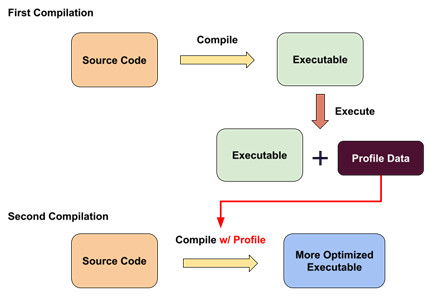
\includegraphics[width=0.9\textwidth]{content/3/chapter12/images/5.png}\\
Figure 12.5 – PGO workflow
\end{center}

Here, the first compilation phase compiled and optimized the code normally. After we executed the compiled program (an arbitrary number of times), we were able to collect the profile data files. In the second compilation phase, we not only optimized the code, as we did previously, but also integrated the profile data into the optimizations to make them act more aggressively. 

There are primarily two ways for PGO to collect runtime profiling data: inserting instrumentation code or leveraging sampling data. Let's introduce both.


\subsubsubsection{12.3.1\hspace{0.2cm}Introduction to instrumentation-based PGO}

Instrumentation-based PGO inserts instrumentation code into the target program during the first compilation phase. This code measures the execution frequency of the program constructions we're interested in – for example, basic blocks and functions – and writes the result in a file. This is similar to how a sanitizer works.

Instrumentation-based PGO usually generates profiling data with higher precision. This is because the compiler can insert instrumentation code in a way that provides the greatest benefit for other optimizations. However, just like the sanitizer, instrumentation-based PGO changes the execution flow of the target program, which increases the risk of performance regression (for the binary that was generated from the first compilation phase).

\subsubsubsection{12.3.2\hspace{0.2cm}Introduction to sampling-based PGO}

Sampling-based PGO uses external tools to collect profiling data. Developers use profilers such as perf or valgrind to diagnose performance issues. These tools usually leverage advanced system features or even hardware features to collect the runtime behavior of a program. For example, perf can give you insights into branch prediction and cache line misses.

Since we are leveraging data from other tools, there is no need to modify the original code to collect profiles. Therefore, sampling-based PGO usually has an extremely low runtime overhead (usually, this is less than 1\%). Also, we don't need to recompile the code for profiling purposes. However, profiling data that's generated in this way is usually less precise. It's also more difficult to map the profiling data back to the original code during the second compilation phase.

In the rest of this section, we are going to focus on instrumentation-based PGO. We are going to learn how to leverage it with LLVM IR. Nevertheless, as we will see shortly, these two PGO strategies in LLVM share lots of common infrastructures, so the code is portable. Here is the list of topics we are going to cover:

\begin{itemize}
\item Working with profiling data
\item Learning about the APIs for accessing profiling data
\end{itemize}

The first topic will show us how to create and use instrumentation-based PGO profiles with Clang, as well as some of the tools that can help us inspect and modify profiling data. The second topic will give you more details on how to access profiling data using LLVM APIs. This is useful if you want to create your own PGO pass.

\hspace*{\fill} \\ %插入空行
\noindent
\textbf{Working with profiling data}

In this section, we are going to learn how to use generate, inspect, and even modify instrumentation-based profiling data. Let's start with the following example:

\begin{lstlisting}[style=styleCXX]
__attribute__((noinline))
void foo(int x) {
	if (get_random() > 5)
	printf("Hello %d\n", x * 3);
}
int main(int argc, char **argv) {
	for (int i = 0; i < argc + 10; ++i) {
		foo(i);
	}
	return 0;
}
\end{lstlisting}

In the preceding code, get\_random is a function that generates a random number from 1 to 10 with uniform distribution. In other words, the highlighted if statement in the foo function should have a 50\% chance of being taken. In addition to the foo function, the trip count of the for loop within main depends on the number of command-line arguments there are.

Now, let's try to build this code with instrumentation-based PGO. Here are the steps:

\begin{enumerate}
\item The first thing we are going to do is generate an executable for PGO profiling. Here is the command:

\begin{tcblisting}{commandshell={}}
$ clang -O1 -fprofile-generate=pgo_prof.dir pgo.cpp -o pgo
\end{tcblisting}

The -fprofile-generate option enables instrumentation-based PGO. The path that we added after this flag is the directory where profiling data will be stored.

\item Next, we must run the pgo program with three command-line arguments:

\begin{tcblisting}{commandshell={}}
$ ./pgo `seq 1 3`
Hello 0
Hello 6
…
Hello 36
Hello 39
$
\end{tcblisting}

You might get a totally different output since there is only a 50\% of chance of  the string being printed.

After this, the pgo\_prof.dir folder should contain the  default\_<hash>\_<n>.profraw file, as shown here:

\begin{tcblisting}{commandshell={}}
$ ls pgo_prof.dir 
default_10799426541722168222_0.profraw
\end{tcblisting}

The hash in the filename is a hash that's calculated based on your code.

\item We cannot directly use the *.profraw file for our second compilation phase. Instead, we must convert it into another kind of binary form using the llvmprofdata tool. Here is the command:

\begin{tcblisting}{commandshell={}}
$ llvm-profdata merge pgo_prof.dir/ -o pgo_prof.profdata
\end{tcblisting}

llvm-profdata is a powerful tool for inspecting, converting, and merging profiling data files. We will look at it in more detail later. In the preceding command, we are merging and converting all the data files under pgo\_prof.dir into a single *.profdata file.

\item Finally, we can use the file we just merged for the second stage of compilation. Here is the command:

\begin{tcblisting}{commandshell={}}
$ clang -O1 -fprofile-use=pgo_prof.profdata pgo.cpp \
        -emit-llvm -S -o pgo.after.ll
\end{tcblisting}

\end{enumerate}

Here, the -fprofile-use option told clang to use the profiling data stored in pgo\_prof.profdata to optimize the code. We are going to look at the LLVM IR code after we've done this optimization.

Open pgo.after.ll and navigate to the foo function. Here is a simplified version
of foo:

\begin{lstlisting}[style=styleCXX]
define void @foo(i32 %x) !prof !71 {
entry:
	%call = call i32 @get_random()
	%cmp = icmp sgt i32 %call, 5
	br i1 %cmp, label %if.then, label %if.end, !prof !72
	
if.then:
	%mul = mul nsw i32 %x, 3
	…
}
\end{lstlisting}

In the preceding LLVM IR code, two places were different from the original IR; that is, the !prof tags that followed after both the function header and the branch instruction, which correspond to the if(get\_random() > 5) code we saw earlier.

In LLVM IR, we can attach metadata to different IR units to provide supplementary information. Metadata will show up as a tag starting with exclamation mark ('!') in the textual LLVM IR.!prof, !71, and !72 in the preceding code are metadata tags that represent the profiling data we collected. More specifically, if we have profiling data associated with an IR unit, it always starts with !prof, followed by another metadata tag that contains the required values. These metadata values are put at the very bottom of the IR file. If we navigate there, we will see the content of !71 and !72. Here is the code:

\begin{tcblisting}{commandshell={}}
!71 = !{!"function_entry_count", i64 110}
!72 = !{!"branch_weights", i32 57, i32 54}
\end{tcblisting}

These two metadata are tuples with two and three elements. !71, as suggested by its first element, represents the number of times the foo function was called (in this case, it was called 110 times).

On the other hand,!72 marks the number of times each branch in the if(get\_ random() > 5) statement was taken. In this case, the true branch was taken 57 times and the false branch was taken 54 times. We got these numbers because we were using uniform distribution for random number generation (namely, a ~50\% chance for each branch).

In the second part of this section, we will learn how to access these values for the sake of developing a more aggressive compiler optimization. Before we do that, though, let's take a deeper look at the profiling data file we just collected.

The llvm-profdata tool we just used can not only help us convert the format of the profiling data, but also gives us a quick preview of its content. The following command prints out the summary for pgo\_prof.profdata, including the profiling values that were collected from every function:

\begin{tcblisting}{commandshell={}}
$ llvm-profdata show –-all-functions –-counts pgo_prof.profdata
…
	foo:
	  Hash: 0x0ae15a44542b0f02
	  Counters: 2
	  Block counts: [54, 57]
	main:
	  Hash: 0x0209aa3e1d398548
	  Counters: 2
	  Block counts: [110, 1]
…
Instrumentation level: IR entry_first = 0
Functions shown: 9
Total functions: 9
Maximum function count: …
Maximum internal block count: …
\end{tcblisting}

Here, we can see the profiling data entries for each function. Each entry has a list of numbers representing the execution frequency of all the enclosing basic blocks.

Alternatively, you can inspect the same profiling data file by converting it into a textual file first. Here is the command:

\begin{tcblisting}{commandshell={}}
$ llvm-profdata merge –-text pgo_prof.profdata -o pgo_prof.
proftext
$ cat pgo_prof.proftext
# IR level Instrumentation Flag
:ir
…
foo
# Func Hash:
784007059655560962
# Num Counters:
2
# Counter Values:
54
57
…
\end{tcblisting}

The *.proftext file is in a human-readable textual format where all the profiling data is simply put in its own line.

This textual representation can actually be converted back into the *.profdata format using a similar command. Here is an example:

\begin{tcblisting}{commandshell={}}
$ llvm-profdata merge –-binary pgo_prof.proftext -o pgo_prof.profdata
\end{tcblisting}

Therefore, *.proftext is especially useful when you want to edit the profiling data manually.

Before we dive into the APIs for PGO, there is one more concept we need to learn about: the instrumentation level.

\hspace*{\fill} \\ %插入空行
\noindent
\textbf{Understanding the instrumentation level}

So far, we've learned that instrumentation-based PGO can insert instrumentation code for collecting runtime profiling data. On top of this fact, the places where we insert this instrumentation code and its granularity also matter. This property is called the instrumentation level in instrumentation-based PGO. LLVM currently supports three different instrumentation levels. Here are descriptions of each:

\begin{itemize}
\item IR: Instrumentation code is inserted based on LLVM IR. For example, the code to collect the number of taken branches is directly inserted before a branch
instruction. The -fprofile-generate command-line option we introduced earlier will generate profiling data with this instrumentation level. For example, let's say we have the following C code:

\begin{lstlisting}[style=styleCXX]
void foo(int x) {
	if (x > 10)
		puts("hello");
	else
		puts("world");
}
\end{lstlisting}

The corresponding IR – without enabling instrumentation-based PGO – is shown here:

\begin{lstlisting}[style=styleCXX]
define void @foo(i32 %0) {
	…
	%4 = icmp sgt i32 %3, 10
	br i1 %4, label %5, label %7
	
5:
	%6 = call i32 @puts(…"hello"…)
	br label %9
7:
	%8 = call i32 @puts(…"world"…)
	br label %9
	
9:
	ret void
}
\end{lstlisting}

As we can see, there is a branch to either basic block; that is, \%5 or \%7. Now, let's generate the IR with instrumentation-based PGO enabled with the following command:

\begin{tcblisting}{commandshell={}}
$ clang -fprofile-generate -emit-llvm -S input.c
\end{tcblisting}

This is the same command we used for the first PGO compilation phase in the Working with profiling data section, except that we are generating LLVM IR instead of an executable. The resulting IR is shown here:

\begin{lstlisting}[style=styleCXX]
define void @foo(i32 %0) {
	…
	%4 = icmp sgt i32 %3, 10
	br i1 %4, label %5, label %9
5:
	%6 = load i64, i64* … @__profc_foo.0, align 8
	%7 = add i64 %6, 1
	store i64 %7, i64* … @__profc_foo.0, align 8
	%8 = call i32 @puts(…"hello"…)
	br label %13
9:
	%10 = load i64, i64* … @__profc_foo.1, align 8
	%11 = add i64 %10, 1
	store i64 %11, i64* … @__profc_foo.1, align 8
	%12 = call i32 @puts(…"world"…)
	br label %13
	
13:
	ret void
}
\end{lstlisting}

In the preceding IR, the basic blocks in both branches have new code in them. More specifically, both increment the value in a global variable – either @\_\_profc\_foo.0 or @\_\_profc\_foo.1 – by one. The values in these two variables will eventually be exported as the profiling data for branches, representing the number of times each branch was taken.

This instrumentation level provides decent precision but suffers from compiler changes. More specifically, if Clang changes the way it emits LLVM IR, the places where the instrumentation code will be inserted will also be different. This effectively means that for the same input code, the profiling data that's generated with an older version of LLVM might be incompatible with the profiling data that's generated with a newer LLVM.

\item AST: Instrumentation code is inserted based on an AST. For example, the code to collect the number of taken branches might be inserted as a new Stmt AST node inside an IfStmt (an AST node). With this method, the instrumentation code is barely affected by compiler changes and we can have a more stable profiling data format across different compiler versions. The downside of this instrumentation level is that it has less precision than the IR instrumentation level.

You can adopt this instrumentation level by simply using the -fprofile-instrgenerate command-line option in place of -fprofile-generate when invoking clang for the first compilation. You don't need to change the command for the second compilation, though.

\item Context-sensitive: In the Working with profiling data section, we learned that we could collect information about the number of times a branch has been taken. However, with the IR instrumentation level, it's nearly impossible to tell which caller function leads to the most branch that has been taken the most. In other words, the conventional IR instrumentation level loses the calling context. The contextsensitive instrumentation level tries to address this problem by collecting the profiles again once the functions have been inlined, thus creating profiling data with higher precision.

However, it's slightly cumbersome to use this feature in Clang – we need to compile the same code three times rather than twice. Here are the steps for using contextsensitive PGO:

\begin{tcblisting}{commandshell={}}
$ clang -fprofile-generate=first_prof foo.c -o foo_exe
$ ./foo_exe …
$ llvm-profdata merge first_prof -o first_prof.profdata
\end{tcblisting}

First, generate some normal (IR instrumentation level) profiling data using what we learned in the Working with profiling data section:

\begin{tcblisting}{commandshell={}}
$ clang -fprofile-use=first_prof.profdata \
        -fcs-profile-generate=second_prof foo.c -o foo_exe2
$ ./foo_exe2
$ llvm-profdata merge first_prof.profdata second_prof \
          -o combined_prof.profdata
\end{tcblisting}

Then, run clang with two PGO command-line options, -fprofile-use and -fcs-profile-generate, with the path to the profiling file from the previous step and the prospective output path, respectively. When we use llvm-profdata to do the post-processing, we are merging all the profiling data files we have:

\begin{tcblisting}{commandshell={}}
$ clang -fprofile-use=combined_prof.profdata \
        foo.c -o optimized_foo
\end{tcblisting}

Finally, feed the combined profiling file into Clang so that it can use this contextsensitive profiling data to get a more accurate portrait of the program's runtime behavior.

\end{itemize}

Note that different instrumentation levels only affect the accuracy of the profiling data; they don't affect how we retrieve this data, which we are going to talk about in the next section.

In the last part of this section, we are going to learn how to access this profiling data inside an LLVM pass via the APIs provided by LLVM.

\hspace*{\fill} \\ %插入空行
\noindent
\textbf{Learning about the APIs for accessing profiling data}

In the previous section, we learned how to run the instrumentation-based PGO using Clang and view the profiling data file using llvm-profdata. In this section, we are going to learn how to access that data within an LLVM pass to help us develop our
own PGO.

Before we go into the development details, let's learn how to consume those profiling data files into opt, since it's easier to test individual LLVM pass using it. Here is a sample command:

\begin{tcblisting}{commandshell={}}
$ opt -pgo-test-profile-file=pgo_prof.profdata \
      --passes="pgo-instr-use,my-pass…" pgo.ll …
\end{tcblisting}

There are two keys in the preceding command:

\begin{itemize}
\item Use -pgo-test-profile-file to designate the profiling data file you want to put in.
\item The "pgo-instr-use" string represents the PGOInstrumentaitonUse pass, which reads (instrumentation-based) profiling files and annotates the data on an LLVM IR. However, it is not run by default, even in the predefined optimization levels (that is, O0 ~ O3, Os, and Oz). Without this pass being ahead in the Pass pipeline, we are unable to access any profiling data. Therefore, we need to explicitly add it to the optimization pipeline. The preceding sample command demonstrated how to run it before a custom LLVM pass, my-pass, in the pipeline. If you want to run it before any of the predefined optimization pipelines – for instance, O1 – you must specify the -\,-passes="pgo-instr-use,default<O1>" command-line option.
\end{itemize}

Now, you might be wondering, what happens after the profiling data is read into opt? It turns out that the LLVM IR file that was generated by the second compilation phase – pgo.after.ll – has provided us with some answers to this question. 

In pgo.after.ll, we saw that some branches were decorated with metadata specifying the number of times they were taken. Similar metadata appeared in functions, which represented the total number of times those functions were called.

More generally speaking, LLVM directly combines the profiling data – read from the file – with its associated IR constructions via metadata. The biggest advantage of this strategy is that we don't need to carry the raw profiling data throughout the entire optimization pipeline – the IR itself contains this profiling information.

Now, the question becomes, how can we access metadata that's been attached to IR? LLVM's metadata can be attached to many kinds of IR units. Let's take a look at the most common one first: accessing metadata attached to an Instruction. The following code shows us how to read the profiling metadata –!prof !71, which we saw previously – that's attached to a branch instruction:

\begin{lstlisting}[style=styleCXX]
// `BB` has the type of `BasicBlock&`
Instruction *BranchInst = BB.getTerminator();
MDNode *BrWeightMD = BranchInst->getMetadata(LLVMContext::MD_
prof);
\end{lstlisting}

In the preceding snippet, we are using BasicBlock::getTerminator to get the last instruction in a basic block, which is a branch instruction most of the time. Then, we tried to retrieve the profiling metadata with the MD\_prof metadata. BrWeightMD is the result we are looking for.
 
The type of BrWeightMD, MDNode, represents a single metadata node. Different MDNode instances can be composed together. More specifically, a MDNode instance can use other MDNode instances as its operands – similar to the Value and User instances we saw in Chapter 10, Processing LLVM IR. The compound MDNode can express more complex concepts.

For example, in this case, each operand in BrWeightMD represents the number of times each branch was taken. Here is the code to access them:

\begin{lstlisting}[style=styleCXX]
if (BrWeightMD->getNumOperands() > 2) {
	// Taken counts for true branch
	MDNode *TrueBranchMD = BrWeightMD->getOperand(1);
	// Taken counts for false branch
	MDNode *FalseBranchMD = BrWeightMD->getOperand(2);
}
\end{lstlisting}

As you can see, the taken counts are also expressed as MDNode.

\begin{tcolorbox}[colback=blue!5!white,colframe=blue!75!black, fonttitle=\bfseries,title=Operand indices for both branches]	
\hspace*{0.7cm}Note that the data for both branches is placed at the operands starting from index 1 rather than index 0.
\end{tcolorbox}

If we want to convert these branch MDNode instances into constants, we can leverage a small utility provided by the mdconst namespace. Here is an example:

\begin{lstlisting}[style=styleCXX]
if (BrWeightMD->getNumOperands() > 2) {
	// Taken counts for true branch
	MDNode *TrueBranchMD = BrWeightMD->getOperand(1);
	ConstantInt *NumTrueBrTaken
	  = mdconst::dyn_extract<ConstantInt>(TrueBranchMD);
	…
}
\end{lstlisting}

The previous code unwrapped an MDNode instance and extracted the underlying ConstantInt instance.

For Function, we can get the number of times it was called in an even easier way. Here is the code:

\begin{lstlisting}[style=styleCXX]
// `F` has the type of `Function&`
Function::ProfileCount EntryCount = F.getEntryCount();
uint64_t EntryCountVal = EntryCount.getCount();
\end{lstlisting}

Function is using a slightly different way to present its called frequency. But retrieving the numerical profiling value is still pretty easy, as shown in the preceding snippet.

It is worth noting that although we only focused on instrumentation-based PGO here, for sampling-based PGO, LLVM also uses the same programming interface to expose its data. In other words, even if you're using profiling data that's been collected from sampling tools with a different opt command, the profiling data will also be annotated on IR units and you can still access it using the aforementioned method. In fact, the tools and APIs we are going to introduce in the rest of this section are mostly profiling-data-source agnostic.

So far, we have been dealing with real values that have been retrieved from the profiling data. However, these low-level values cannot help us go far in terms of developing a compiler optimization or program analysis algorithm – usually, we are more interested in high-level concepts such as "functions that are executed most frequently" or "branches that are least taken". To address these demands, LLVM builds several analyses on top of profiling data to deliver such high-level, structural information.

In the next section, we are going to introduce some of these analyses and their usages in LLVM Pass.

\subsubsubsection{12.3.3\hspace{0.2cm}Using profiling data analyses}

In this section, we are going to learn three analysis classes that can help us reason about the execution frequency of basic blocks and functions at runtime. They are as follows:

\begin{itemize}
\ttfamily
\item BranchProbabilityInfo
\item BlockFrequencyInfo
\item ProfileSummaryInfo
\end{itemize}

This list is ordered by their analyzing scope in the IR – from local to global. Let's start with the first two.

\hspace*{\fill} \\ %插入空行
\noindent
\textbf{Using BranchProbabilityInfo and BlockFrequencyInfo}

In the previous section, we learned how to access the profiling metadata that's attached to each branch instruction – the branch weight. The analysis framework in LLVM provides you with an even easier way to access these values via the BranchProbabilityInfo class. Here is some example code showing how to use it in a (function) Pass:

\begin{lstlisting}[style=styleCXX]
#include "llvm/Analysis/BranchProbabilityInfo.h"
PreservedAnalyses run(Function &F, FunctionAnalysisManager
&FAM) {
	BranchProbabilityInfo &BPI
	  = FAM.getResult<BranchProbabilityAnalysis>(F);
	BasicBlock *Entry = F.getEntryBlock();
	BranchProbability BP = BPI.getEdgeProbability(Entry, 0);
	…
}
\end{lstlisting}

The previous code retrieved a BranchProbabilityInfo instance, which is the result of BranchProbabilityAnalysis, and tried to get the weight from the entry block to its first successor block.

The returned value, a BranchProbability instance, gives you the branch's probability in the form of a percentage. You can use BranchProbability::getNumerator to retrieve the value (the "denominator" is 100 by default). The BranchProbability class also provides some handy utility methods for performing arithmetic between two branch probabilities or scaling the probability by a specific factor. Although we can easily tell which branch is more likely to be taken using BranchProbabilityInfo, without additional data, we can't tell the branch's probability (to be taken) in the whole function. For example, let's assume we have the following CFG:

\hspace*{\fill} \\ %插入空行
\begin{center}
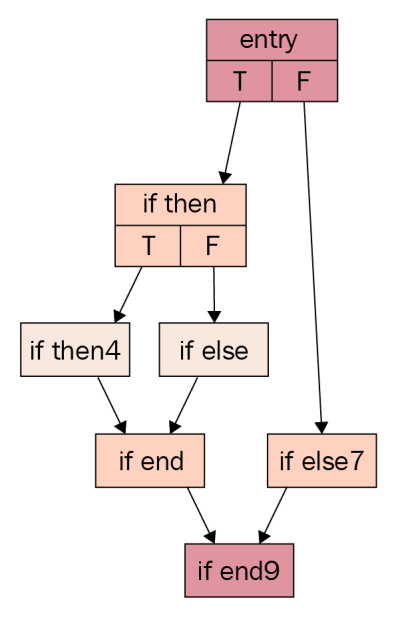
\includegraphics[width=0.3\textwidth]{content/3/chapter12/images/6.png}\\
Figure 12.6 – CFG with nested branches
\end{center}

For the preceding diagram, we have profiling counter values for the following basic blocks:

\begin{itemize}
\item if.then4: 2
\item if.else: 10
\item if.else7: 20
\end{itemize}

If we only look at the branch weight metadata toward blocks if.then4 and if.else – that is, the true and false branches for if.then, respectively – we might come under the illusion that the if.else block has a ~83\% chance of being taken. But the truth is, it only has a ~31\% chance because the control flow has a higher probability to go into if.else7 before even entering the if.then region. Of course, in this case, we can do simple math to figure out the correct answer, but when the CFG is getting bigger and more complex, we might have a hard time doing this by ourselves.

The BlockFrequencyInfo class provides a shortcut to this problem. It can tell us the frequency of each basic block to be taken under the context of its enclosing function. Here is an example of its usage in a Pass:

\begin{lstlisting}[style=styleCXX]
#include "llvm/Analysis/BlockFrequencyInfo.h"
PreservedAnalyses run(Function &F, FunctionAnalysisManager
&FAM) {
	BlockFrequencyInfo &BFI
	  = FAM.getResult<BlockFrequencyAnalysis>(F);
	for (BasicBlock *BB : F) {
		BlockFrequency BF = BFI.getBlockFreq(BB);
	}
	…
}
\end{lstlisting}

The previous code retrieved a BlockFrequencyInfo instance, which is the result of BlockFrequencyAnalysis, and tried to evaluate the block frequency of each basic block in the function.

Similar to the BranchProbability class, BlockFrequency also provides nice utility methods to calculate with other BlockFrequency instances. But different from BranchProbability, the numeric value that's retrieved from BlockFrequency is not presented as a percentage. More specifically, BlockFrequency::getFrequency returns an integer that is the frequency relative to the entry block of the current function. In other words, to get a percentage-based frequency, we can use the following snippet:

\begin{lstlisting}[style=styleCXX]
// `BB` has the type of `BasicBlock*`
// `Entry` has the type of `BasicBlock*` and represents entry
// block
BlockFrequency BBFreq = BFI.getBlockFreq(BB),
               EntryFreq = BFI.getBlockFreq(Entry);
auto FreqInPercent
  = (BBFreq.getFrequency() / EntryFreq.getFrequency()) * 100;
\end{lstlisting}

The highlighted FreqInPercent is the block frequency of BB, expressed as a percentage.

BlockFrequencyInfo calculates the frequency of a specific basic block under the context of a function – but what about the entire module? More specifically, if we bring a call graph into this situation, can we multiply the block frequency we just learned with the frequency of the enclosing function being called, in order to get the execution frequency in the global scope? Fortunately, LLVM has prepared a useful class to answer this question – ProfileSummaryInfo.

\hspace*{\fill} \\ %插入空行
\noindent
\textbf{Using ProfileSummaryInfo}

The ProfileSummaryInfo class gives you a global view of all the profiling data in a Module. Here is an example of retrieving an instance of it inside a module Pass:

\begin{lstlisting}[style=styleCXX]
#include "llvm/Analysis/ProfileSummaryInfo.h"
PreservedAnalyses run(Module &M, ModuleAnalysisManager &MAM) {
	ProfileSummaryInfo &PSI = MAM.
	getResult<ProfileSummaryAnalysis>(M);
	…
}
\end{lstlisting}

ProfileSummaryInfo provides a wide variety of functionalities. Let's take a look at three of its most interesting methods:

\begin{itemize}
\item isFunctionEntryCold/Hot(Function*): These two methods compare the entry count of a Function – which effectively reflects the number of times a function was called –against that of other functions in the same module and tell us if the inquiry function is ranking high or low in this metric.

\item isHot/ColdBlock(BasicBlock*, BlockFrequencyInfo\&): These two methods work similarly to the previous bullet one but compare the execution frequency of a BasicBlock against all the other blocks in the module.

\item isFunctionCold/HotInCallGraph(Function*,
BlockFrequencyInfo\&): These two methods combine the methods from the previous two bullet points they can tell you whether a function is considered hot or cold based on its entry count or the execution frequency of its enclosing basic blocks. This is useful when a function has a low entry count – that is, it was not called often – but contains a loop that has extremely a high basic block execution frequency. In this case, the isFunctionHotInCallGraph method can give us a more accurate assessment.

\end{itemize}

These APIs also have variants where you can designate the cutoff point as being "hot" or "cold." Please refer to the API documentation for more information.

For a long time, the compiler was only able to analyze and optimize the source code with a static view. For dynamic factors inside a program – for instance, the branch taken count – compilers could only make an approximation. PGO opened an alternative path to provide extra information for compilers to peek into the target program's runtime behavior, for the sake of making less ambiguous and more aggressive decisions. In this section, we learned how to collect and use runtime profiling information – the key to PGO – with LLVM. We learned how to use the related infrastructure in LLVM to collect and generate such profiling data. We also learned about the programming interface we can use to access that data – as well as some high-level analyses built on top of it – to assist our development inside an LLVM Pass. With these abilities, LLVM developers can plug in this runtime information to further improve the quality and precision of their existing optimization Passes.














